\subsubsection{Ý tưởng}
Insertion sort là một thuật toán sắp xếp đơn giản hoạt động bằng cách lặp lại việc chèn từng phần tử của một danh sách chưa được sắp xếp vào đúng vị trí của nó trong một phần đã được sắp xếp của danh sách. Nó giống như việc sắp xếp các lá bài trong tay bạn. Bạn chia các lá bài thành hai nhóm: các lá bài đã được sắp xếp và các lá bài chưa được sắp xếp. Sau đó, bạn chọn một lá bài từ nhóm chưa được sắp xếp và đặt nó vào đúng vị trí trong nhóm đã được sắp xếp. \cite{smith2022insertion}
\subsubsection{Mã giả}

\begin{algorithm}[H]
\caption{Insertion sort}
\begin{algorithmic}[1]
\Procedure{Insertion sort}{$arr, n$}
    \State \textbf{Input:} Mảng $arr$ gồm $n$ phần tử
    \State \textbf{Output:} Mảng $arr$ được sắp xếp
    
    \For{$i \gets 1$ to $n-1$}
    \State $key \gets arr[i]$
    \State $j \gets i - 1$
    \While{$j \geq 0$ \textbf{and} $arr[j] > key$}
        \State $arr[j+1] \gets arr[j]$
        \State $j \gets j - 1$
    \EndWhile
    \State $arr[j+1] \gets key$
\EndFor
\EndProcedure
\end{algorithmic}
\end{algorithm}

\subsubsection{Ví dụ}
Giả sử chúng ta có mảng ban đầu: $[42, 17, 93, 58, 21, 76, 34]$. Dưới đây là các bước thực hiện Insertion sort minh họa bằng hình ảnh:


\begin{figure}[H]
    \centering
    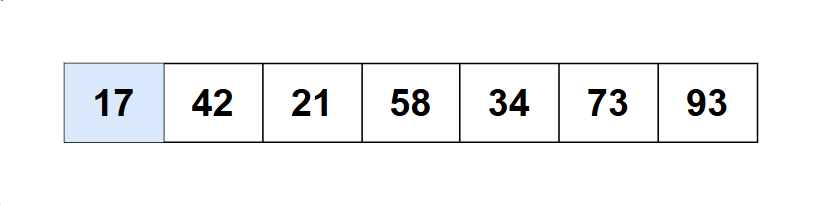
\includegraphics[width=0.7\textwidth]{img/insertion sort_lan2/1.png}
    
\end{figure}
\newpage

\begin{itemize}
    \item Chúng ta bắt đầu với phần tử thứ hai của mảng vì phần tử đầu tiên trong mảng được coi là đã được sắp xếp.
    \begin{figure}[H]
        \centering
        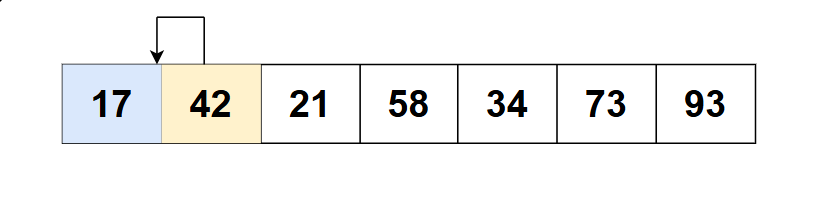
\includegraphics[width=0.7\textwidth]{img/insertion sort_lan2/2.png}

    \end{figure}
    
\end{itemize}


\begin{itemize}
    \item So sánh phần tử thứ hai với phần tử thứ nhất và kiểm tra xem phần tử thứ hai có nhỏ hơn không, nếu có thì hoán đổi chúng.

    \begin{figure}[H]
        \centering
        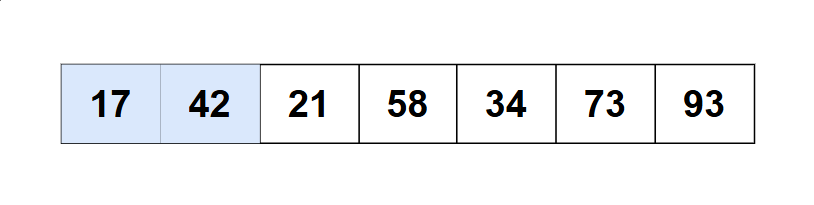
\includegraphics[width=0.7\textwidth]{img/insertion sort_lan2/3.png}
\caption{kết quả việc so sánh và hoán vị.}
    \end{figure}
    
\end{itemize}

\begin{itemize}
    \item Di chuyển đến phần tử thứ ba và so sánh nó với hai phần tử đầu tiên và đặt vào đúng vị trí của nó sao cho giữ đúng tính chất sắp xếp
    \begin{figure}[H]
        \centering
        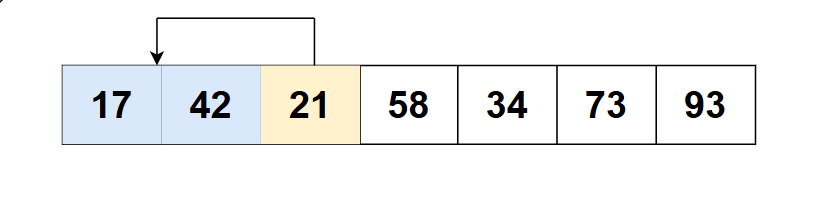
\includegraphics[width=0.7\textwidth]{img/insertion sort_lan2/4.png}
        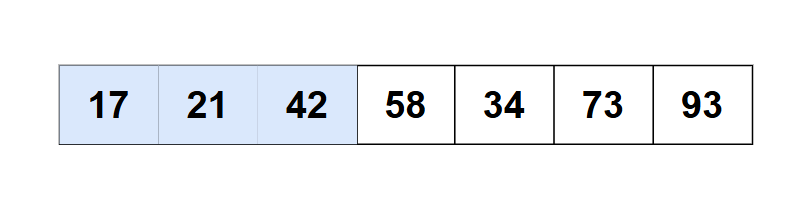
\includegraphics[width=0.7\textwidth]{img/insertion sort_lan2/5.png}
         \caption{kết quả sau khi chèn đúng vị trí.}
    \end{figure}
    
\end{itemize}

\newpage

\begin{itemize}
\item Tiếp tục, cứ lấy phần tử kế tiếp chèn vào đúng vị trí trong mảng con màu xanh phía trước. Lặp lại cho đến khi toàn bộ mảng được sắp xếp
    \begin{figure}[H]
        \centering
        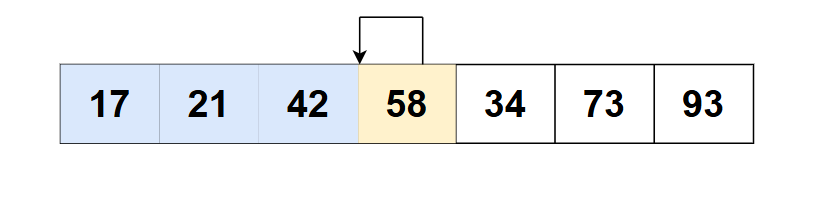
\includegraphics[width=0.7\textwidth]{img/insertion sort_lan2/6.png}
    \end{figure}

    \begin{figure}[H]
        \centering
        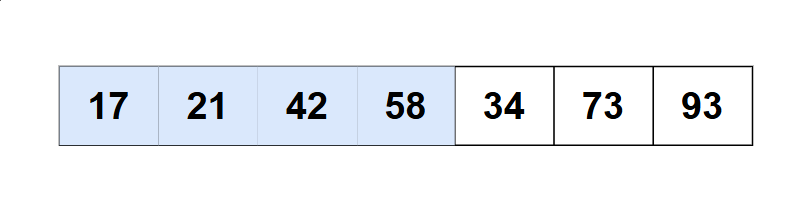
\includegraphics[width=0.7\textwidth]{img/insertion sort_lan2/7.png}
    \end{figure}

    \begin{figure}[H]
        \centering
        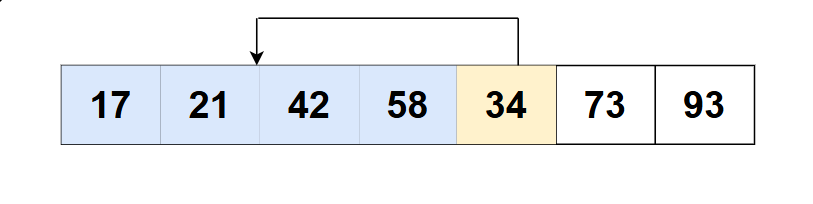
\includegraphics[width=0.7\textwidth]{img/insertion sort_lan2/8.png}
    \end{figure}
    
    \begin{figure}[H]
        \centering
        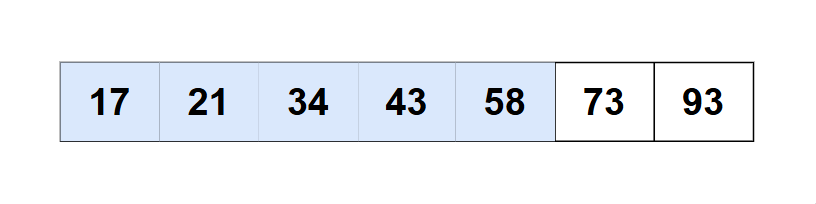
\includegraphics[width=0.7\textwidth]{img/insertion sort_lan2/9.png}
    \end{figure}

    \begin{figure}[H]
        \centering
        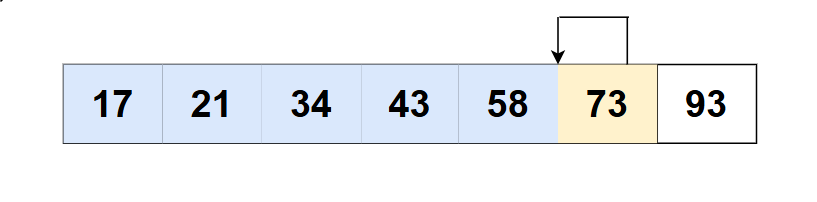
\includegraphics[width=0.7\textwidth]{img/insertion sort_lan2/10.png}
    \end{figure}

    \begin{figure}[H]
        \centering
        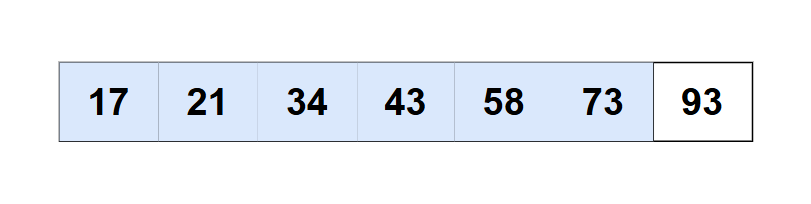
\includegraphics[width=0.7\textwidth]{img/insertion sort_lan2/11.png}
    \end{figure}

    \begin{figure}[H]
        \centering
        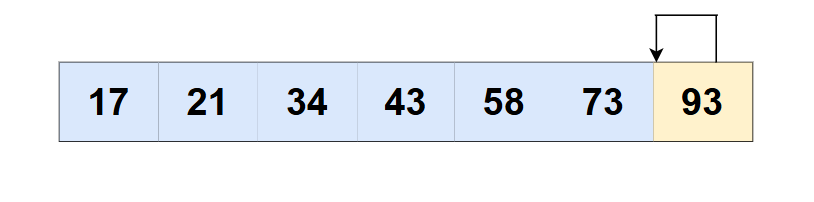
\includegraphics[width=0.7\textwidth]{img/insertion sort_lan2/12.png}
    \end{figure}

    \begin{figure}[H]
        \centering
        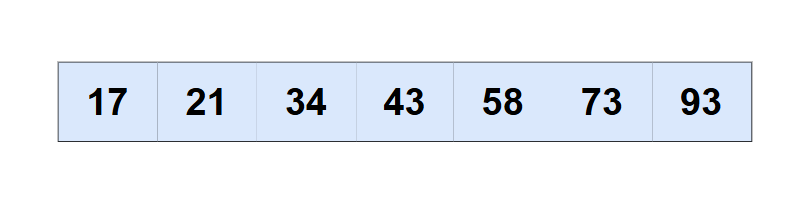
\includegraphics[width=0.7\textwidth]{img/insertion sort_lan2/13.png}
        \caption{Mảng đã được sắp xếp.}
    \end{figure}
\end{itemize}




\subsubsection{{Độ phức tạp}}
\begin{itemize}
    \item[\textbf{--}] {Thời gian:}
    \begin{itemize}
        \item[$\bullet$] \textbf{Best Case:} \(\mathcal{O}(n)\), xảy ra khi mảng đã được sắp xếp. Trong trường hợp này, mỗi phần tử chỉ cần được so sánh một lần và không có phép chèn nào thực hiện.
        \item[$\bullet$] \textbf{Average Case:} \(\mathcal{O}(n^2)\), xảy ra khi các phần tử trong mảng được phân bố ngẫu nhiên. Số lần so sánh và chèn tăng dần theo kích thước của mảng.
        \item[$\bullet$] \textbf{Worst Case:} \(\mathcal{O}(n^2)\), xảy ra khi mảng được sắp xếp theo thứ tự ngược lại. Trong trường hợp này, mỗi phần tử cần được so sánh với tất cả các phần tử trước đó và được chèn vào đầu danh sách.
    \end{itemize}
    \item[\textbf{--}] {Không gian:}
    \begin{itemize}
        \item[$\bullet$] Insertion Sort là một thuật toán \textbf{không yêu cầu bộ nhớ bổ sung} (\textbf{in-place}), vì nó thực hiện sắp xếp trực tiếp trên mảng đầu vào.
        \item[$\bullet$] Độ phức tạp bộ nhớ là:
        \[
        \mathcal{O}(1)
        \]
    \end{itemize}
    \item[\textbf{--}] {Tính ổn định:}
    \begin{itemize}
        \item[$\bullet$] Insertion Sort là một thuật toán \textbf{ổn định}. Khi hai phần tử có giá trị bằng nhau, thứ tự ban đầu của chúng được bảo toàn sau quá trình sắp xếp.
    \end{itemize}
\end{itemize}
